%Code by GVV Sharma
%December 9, 2019
%released under GNU GPL
%Locating the circumcentre

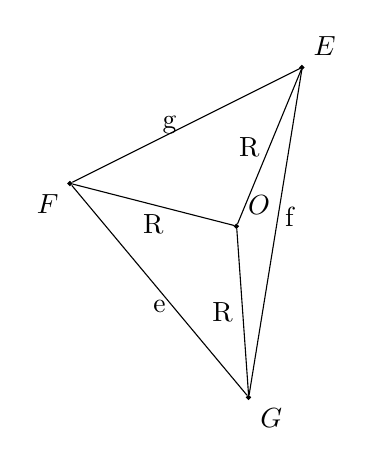
\begin{tikzpicture}
[scale=3.5,>=stealth,point/.style={draw,circle,fill = black,inner sep=0.5pt},]

%Triangle sides
\def\e{1.010}
\def\f{1.212}
\def\g{0.940}
 
%Coordinates of A
%\def\p{{\a^2+\c^2-\b^2}/{(2*\a)}}
%\def\p{0.5}
%\def\q{{sqrt(\c^2-\p^2)}}

%Labeling points
\node (E) at (5.313,2.657)[point,label=above right:$E$] {};
\node (F) at (4.471,2.236)[point,label=below left:$F$] {};
\node (G) at (5.119,1.460)[point,label=below right:$G$] {};

%Circumcentre

\node (O) at (5.075,2.081)[point,label=above right:$O$] {};

%Drawing triangle EFG
\draw (E) -- node[left] {$\textrm{g}$} (F) -- node[below] {$\textrm{e}$} (G) -- node[right,yshift=2mm] {$\textrm{f}$} (E);
%Drawing OA, OB, OC
\draw (O) -- node[left] {$\textrm{R}$} (E);
\draw (O) -- node[below] {$\textrm{R}$} (F);
\draw (O) -- node[left] {$\textrm{R}$} (G);

%\tkzMarkAngle[fill=blue!50,size=.3](C,B,O)
%\tkzMarkAngle[fill=blue!50,size=.3](O,C,B)


%\tkzMarkAngle[fill=red!50](O,A,C)
%\tkzMarkAngle[fill=red!50](A,C,O)


%\tkzMarkAngle[fill=orange!50,size=.3](B,A,O)
%\tkzMarkAngle[fill=orange!50,size=.3](O,B,A)

%\tkzLabelAngle[pos=0.5](O,C,B){$\theta_1$}
%\tkzLabelAngle[pos=0.5](O,B,C){$\theta_1$}
%\tkzLabelAngle[pos=0.5](O,A,B){$\theta_2$}
%\tkzLabelAngle[pos=0.5](O,B,A){$\theta_2$}
%\tkzLabelAngle[pos=1.5](O,A,C){$\theta_3$}
%\tkzLabelAngle[pos=1.5](O,C,A){$\theta_3$}

\end{tikzpicture}
